
\phantomsection
\section{Modifications to D2}

\phantomsection
\addcontentsline{toc}{subsection}{UC2. Create Insurance Policy}
\hypertarget{UC2}{}
\usecaseheader
  {UC2}  % 1: ID
  {Create Insurance Policy} % 2: Titolo
  {To enable the System Administrator to create new insurance policies shared across all facilities in the healthcare
network.} % 3: Goal
  {Scope: Global Insurance Policy handling. Level: Primary.} % 4: Scope
  {The user is logged in as a System Admin.} % 5: Preconditions
  {A new Insurance Policy is created.} % 6: Success
  {The System remains unchanged. The System returns an error.} % 7: Failed
  {Primary: System Admin. Secondary: Database.} % 8: Actors
  {The System Admin asks the System to create a new Insurance Policy.} % 9: Trigger
\begin{ucrequirements}
    FR9.1 & Create insurance policy \\ \hline
    NFR4 & Scalability and capacity \\ \hline     
\end{ucrequirements}
\begin{ucflow}
    1 & The System Admin asks the System to create a new Insurance Policy. \\ \hline
    2 & The System Admin fills in the required fields. \\ \hline
    3 & The System Admin saves. \\ \hline
    4 & The System checks if the discount percentage is a valid amount. \\ \hline
    5 & \hl{The System checks if the maximum coverage is a valid amount.} \\\hline
    6 & The System creates the new Insurance Policy in the Database. \\ \hline
    7 & The System returns a success message. \\ \hline
\end{ucflow}

\begin{ucextensions}
    3a & \textbf{The System Admin cancels:}\newline 
         1. The System aborts the creation process.\newline 
         2. Use case ends. \\ \hline
    4a & \textbf{Validity check fails:}\newline 
         1. The System identifies an invalid amount for the discount percentage.\newline 
         2. The System returns an error.\newline 
         3. Go to main flow step 2 to perform a correction. \\ \hline
    \rowcolor{yellow}
    5a & \textbf{Validity check fails:}\newline 
         1. The System identifies an invalid amount for the maximum coverage.\newline 
         2. The System returns an error.\newline 
         3. Go to main flow step 2 to perform a correction. \\ \hline
\end{ucextensions}
\begin{ucedits}
Added a backend validity check for the maximum coverage amount (steps 5 and 5a). 
The check was already implemented in the system but had not been explicitly documented in this use case.
\end{ucedits}


\phantomsection
\addcontentsline{toc}{subsection}{UC6. Update Insurance Policy}
\hypertarget{UC6}{}
\usecaseheader
  {UC6}  % 1: ID
  {Update Insurance Policy} % 2: Titolo
  {To enable the System Administrator to edit an existing insurance policies shared across all facilities in the healthcare
network.} % 3: Goal
  {Scope: Global Insurance Policy handling. Level: Primary.} % 4: Scope
  {The user is logged in as a System Admin.} % 5: Preconditions
  {An existing Insurance Policy is edited.} % 6: Success
  {The System remains unchanged. The System returns an error.} % 7: Failed
  {Primary: System Admin. Secondary: Database.} % 8: Actors
  {The System Admin asks the System to edit an existing Insurance Policy.} % 9: Trigger
\begin{ucrequirements}
        FR9.3 & Update insurance policy \\ \hline 
\end{ucrequirements}
\begin{ucflow}
    1 & The System Admin asks the System to update an existing Insurance Policy. \\ \hline
    2 & The System Admin fills in the required fields. \\ \hline
    3 & The System Admin saves. \\ \hline
    4 & The System checks if the discount percentage is a valid amount. \\ \hline
    5 & \hl{The System checks if the maximum coverage is a valid amount.} \\\hline
    6 & The System updates the Insurance Policy in the Database. \\ \hline
    7 & The System returns a success message. \\ \hline
\end{ucflow}

\begin{ucextensions}
    3a & \textbf{The System Admin cancels:}\newline 
         1. The System aborts the editing process.\newline 
         2. Use case ends. \\ \hline
    4a & \textbf{Validity check fails:}\newline 
         1. The System identifies an invalid amount for the discount percentage.\newline 
         2. The System returns an error.\newline 
         3. Go to main flow step 2 to perform a correction. \\ \hline
    
    \rowcolor{yellow}
    5a & \textbf{Validity check fails:}\newline 
         1. The System identifies an invalid amount for the maximum coverage.\newline 
         2. The System returns an error.\newline 
         3. Go to main flow step 2 to perform a correction. \\ \hline
\end{ucextensions}
\begin{ucedits}
Added a backend validity check for the maximum coverage amount (steps 5 and 5a). The check was already implemented during Insurance Policy updates but had not been explicitly documented in this use case.
\end{ucedits}

\phantomsection
\addcontentsline{toc}{subsection}{UC10. Cancel appointment (Patient)}
\hypertarget{UC10}{}
\usecaseheader
  {UC10}  % 1: ID
  {Cancel appointment (Patient)} % 2: Titolo
  {To enable Patient to cancel a booked medical appointment} % 3: Goal
  {Scope: Appointment management. Level: Primary.} % 4: Scope
  {The Patient is logged in.} % 5: Preconditions
  {An existing medical appointment is deleted.} % 6: Success
  {The System remains unchanged. The System returns an error.} % 7: Failed
  {Primary: Patient. Secondary: Database, Payment Service, Mail Service.} % 8: Actors
  {Patient asks the System to cancel a booked appointment.} % 9: Trigger
\begin{ucrequirements}
    FR16.2 & Cancel appointment (Patient) \\ \hline
    \end{ucrequirements}
\begin{ucflow}
    1 & Patient asks the System to cancel a booked appointment. \\ \hline
    2 & The System asks for confirmation. \\ \hline
    3 & The Patient confirms. \\ \hline
    4 & The System performs validity check. \\ \hline
    5 & The System cancels the appointment. \\ \hline
    6 & The Patient is refunded. \\\hline
    7 & \hl{The System sends a cancellation email.} \\\hline
\end{ucflow}

\begin{ucextensions}
    3a & \textbf{The Patient cancels:}\newline 
         1. The System aborts the editing process.\newline 
         2. Use case ends. \\ \hline
    4a & \textbf{Late canceling:}\newline 
         1. The System identifies that the appointment is in less than 48 hours.\newline 
         2. Cancellation is aborted.\newline 
         3. The System returns an error.\newline 
         4. Use case ends. \\ \hline
    6a & \textbf{Appointment not paid:}\newline 
         1. The System checks if the appointment was paid ahead.\newline 
         2. If not, proceed to step 7 (refund is skipped).\\ \hline
\end{ucextensions}
\begin{ucedits}
Added the appointment cancellation email notification (step 7) to align the use case with the actual system behavior and ensure that patient communications are explicitly documented.
\end{ucedits}

\phantomsection
\addcontentsline{toc}{subsection}{UC12. Register Doctor}
\hypertarget{UC12}{}
\usecaseheader
  {UC12} % 1: ID
  {Register Doctor} % 2: Titolo
  {A System Admin wants to add a new Doctor to the hospital’s digital infrastructure.} % 3: Goal
  {Scope: Hospital structures handling. Level: Primary.} % 4: Scope
  {The user is logged in as a System Admin. \sout{The relevant hospital structure already exists.}} % 5: Preconditions
  {The Doctor is successfully saved in the Database, and a set of one-time credentials is provided to the System Admin.} % 6: Success
  {The registration is aborted due to invalid data or duplication; no credentials are created.} % 7: Failed
  {Primary: System Admin. Secondary: Database.} % 8: Actors
  {The System Admin asks the System to create a new Doctor account.} % 9: Trigger

\begin{ucrequirements}
    FR1.7 & Doctor registration \\ \hline
    NFR4 & Scalability and capacity \\ \hline
\end{ucrequirements}

\begin{ucflow}
    1 & The System Admin asks the System to create a new Doctor account. \\ \hline
    2 & The System Admin fills in the required fields, including Doctor's personal data. \\ \hline
    3 & The System Admin saves. \\ \hline
    4 & The System checks if the \hl{fiscal code} field is not duplicate. \\ \hline
    5 & The System creates the new Doctor account in the Database. \\ \hline
    6 & The System returns the new account credentials, which are displayed just once. \\ \hline
\end{ucflow}

\begin{ucextensions}
    3a & \textbf{The System Admin cancels:}\newline 
         1. The System aborts the creation process.\newline 
         2. Use case ends. \\ \hline
    4a & \textbf{Validity check fails:}\newline 
         1. The System identifies duplicated personal data for the Doctor.\newline 
         2. The System returns an error.\newline 
         3. Go to main flow step 2 to perform a correction. \\ \hline
\end{ucextensions}

\begin{ucedits}
Removed the precondition requiring the relevant hospital structure to already exist, as it is not necessary for Doctor registration. 
Replaced the uniqueness check from "name" to "fiscal code" to correctly identify duplicate Doctor records using a unique identifier.
\end{ucedits}

\phantomsection
\addcontentsline{toc}{subsection}{UC13. Assign Doctor to Hospital}
\hypertarget{UC13}{}
\usecaseheader
  {UC13} % 1: ID
  {Assign Doctor to Hospital} % 2: Titolo
  {To enable the System Administrator to assign a registered Doctors to a specific hospital.} % 3: Goal
  {Scope: Hospital structures handling. Level: Primary.} % 4: Scope
  {The user is logged in as a System Admin. The target hospital exists. The Doctors are registered in the System.} % 5: Preconditions
  {The selected Doctors are successfully assigned to the selected hospital.} % 6: Success
  {The assignment fails; previous assignments remain unchanged.} % 7: Failed
  {Primary: System Admin, Head of Hospital. Secondary: Database.} % 8: Actors
  {The user selects Doctors and assigns them to a hospital.} % 9: Trigger


\begin{ucrequirements}
    FR1.8 & Doctor assignment \\ \hline
    NFR4 & Scalability and capacity \\ \hline
\end{ucrequirements}


\begin{ucflow}
    1 & The System Admin selects one or more Doctors from the set of registered Doctors. \\ \hline
    2 & The System Admin selects the target hospital. \\ \hline
    3 & The System Admin requests assignment. \\ \hline
    4 & The System checks whether selected Doctors are already assigned to a hospital. \\ \hline
    5 & The System displays current assignment status (including any existing hospital assignments). \\ \hline
    6 & The System Admin confirms or modifies the selection. \\ \hline
    7 & The System assigns the Doctors to the selected hospital and updates the System status. \\ \hline
\end{ucflow}


\begin{ucextensions}
    3a & \textbf{Cancel operation:}\newline 
         1. The System Admin cancels the assignment.\newline 
         2. No changes are made to the System.\newline 
         3. Use case ends. \\ \hline

    6a & \textbf{System Admin does not confirm assignment:}\newline 
         1. The System Admin rejects the proposed assignment or modifies the selection.\newline 
         2. The System returns to step 1 or 2 depending on modification.\newline 
         3. Use case continues or ends. \\ \hline
\end{ucextensions}


\begin{ucedits}
Moved validity checking of existing assignments before confirmation, so the System Admin is informed of current Doctor allocation status prior to final confirmation.
\end{ucedits}   


\phantomsection
\addcontentsline{toc}{subsection}{UC14. Appoint Head of Hospital}
\hypertarget{UC14}{}
\usecaseheader
  {UC14} % 1: ID
  {Appoint Head of Hospital} % 2: Titolo
  {To enable the System Administrator to appoint a Registered Doctor to the strategic role of Head of Hospital for a specific facility.} % 3: Goal
  {Scope: Hospital structures handling. Level: Primary.} % 4: Scope
  {The user is logged in as a System Administrator. The specific hospital has been created. The Doctor is already registered in the System.} % 5: Preconditions
  {The selected Doctor is successfully appointed as Head of Hospital.} % 6: Success
  {The appointment fails; the System state remains unchanged and the previous head (if any) remains in place.} % 7: Failed
  {Primary: System Administrator. Secondary: Database.} % 8: Actors
  {The System Administrator wants to appoint a Doctor as Head of Hospital.} % 9: Trigger


\begin{ucrequirements}
    FR2 & Strategic role appointment (Head of Hospital) \\ \hline
\end{ucrequirements}


\begin{ucflow}
    1 & The System Administrator selects a Doctor from the list of Registered Doctors. \\ \hline
    2 & The Admin saves the selection. \\ \hline
    3 & The System prompts a confirmation message including the currently assigned Head of Hospital (if any). \\ \hline
    4 & The Admin confirms the replacement. \\ \hline
    5 & The System performs validity checks. \\ \hline
    6 & The Doctor is appointed as Head of Hospital and the System status is updated. \\ \hline
\end{ucflow}


\begin{ucextensions}
    2a & \textbf{Operation canceled:}\newline 
         1. Admin cancels the operation.\newline 
         2. No changes are made to the Database.\newline 
         3. Use case ends. \\ \hline

    5a & \textbf{Doctor not found:}\newline 
         1. System cannot find the selected Doctor.\newline 
         2. Operation is aborted.\newline 
         3. System returns an error.\newline 
         4. Use case ends. \\ \hline
\end{ucextensions}


\begin{ucedits}
Removed extension 2a ("Already existing Head of Hospital") because it is redundant: the System now displays the current Head of Hospital during the confirmation step, and the Admin implicitly confirms the replacement.
Adjusted the main flow so that role replacement is handled entirely within the confirmation step.
\end{ucedits}
\phantomsection
\addcontentsline{toc}{subsection}{UC15. Appoint Head of Department}
\hypertarget{UC15}{}
\usecaseheader
  {UC15} % 1: ID
  {Appoint Head of Department} % 2: Titolo
  {To enable the Head of Hospital to appoint a Registered Doctor to the tactical role of Head of Department within their facility.} % 3: Goal
  {Scope: Hospital structures handling. Level: Primary.} % 4: Scope
  {The user is logged as a Head of Hospital. The specific department has been created. The Doctor is registered in the System.} % 5: Preconditions
  {The selected Doctor is successfully appointed as Head of Department.} % 6: Success
  {Head of Department appointment fails. The System remains unchanged.} % 7: Failed
  {Primary: Head of Hospital. Secondary: Database.} % 8: Actors
  {The Head of Hospital wants to appoint a Doctor as Head of Department.} % 9: Trigger


\begin{ucrequirements}
    FR3 & Tactical role appointment (Head of Department) \\ \hline
\end{ucrequirements}


\begin{ucflow}
    1 & The Head of Hospital selects a Doctor from the set of Registered Doctors in their facility. \\ \hline
    2 & The Head of Hospital saves the selection. \\ \hline
    3 & The System prompts a confirmation message including the currently assigned Head of Department (if any). \\ \hline
    4 & The Head of Hospital confirms the replacement. \\ \hline
    5 & The System performs validity checks. \\ \hline
    6 & The Doctor is appointed as Head of Department and the System status is updated. \\ \hline
\end{ucflow}


\begin{ucextensions}
    2a & \textbf{Operation canceled:}\newline 
         1. Head of Hospital cancels the operation.\newline 
         2. No changes are made to the Database.\newline 
         3. Use case ends. \\ \hline

    5a & \textbf{Doctor not found:}\newline 
         1. System cannot find the selected Doctor.\newline 
         2. Operation is aborted.\newline 
         3. System returns an error.\newline 
         4. Use case ends. \\ \hline
\end{ucextensions}


\begin{ucedits}
Removed extension 2a ("Already existing Head of Department") because it is redundant: the System now displays the current Head of Department during the confirmation step, and the Head of Hospital implicitly confirms the replacement when proceeding.
Adjusted the main flow so that role replacement is handled entirely within the confirmation step.
\end{ucedits}

\phantomsection
\addcontentsline{toc}{subsection}{UC23. Patient registration and validation}
\hypertarget{UC23}{}
\usecaseheader
  {UC23} % 1: ID
  {\hl{Patient} registration and validation} % 2: Titolo
  {To allow an Unregistered Patient to create and validate an account within the System} % 3: Goal
  {Scope: Users account management. Level: Primary Task.} % 4: Scope
  {The Patient is not authenticated and does not have an active account.} % 5: Preconditions
  {A new account is registered in the System and successfully validated.} % 6: Success
  {No new account is created, or the account remains unverified; the user is prompted with an error message.} % 7: Failed
  {Primary: Patient. Secondary: Database, Mail Service, Identity Provider (SPID/CIE).} % 8: Actors
  {The Unregistered Patient wants to register in the System.} % 9: Trigger


\begin{ucrequirements}
    FR11.1 & User registration \\ \hline
    FR11.2 & User validation \\ \hline
    NFR0 & Security and privacy \\ \hline
    NFR6 & SPID/CIE-based registration and authentication \\ \hline
    NFR7 & Login validity period \\ \hline
\end{ucrequirements}


\begin{ucflow}
    1 & The System asks the Unregistered Patient to insert their email and personal information. \\ \hline
    2 & The Patient fills in the required information. \\ \hline
    3 & The Unregistered Patient submits. \\ \hline
    4 & The System validates the input fields. \\ \hline
    5 & The Patient submits personal information together with the password. \\ \hline
    6 & The System checks password security (complexity and strength). \\ \hline
    7 & The System creates a new unverified account in the Database. \\ \hline
    8 & The System sends a verification token to the provided email address via the Mail Service. \\ \hline
    9 & The User accesses their mailbox and clicks on the validation link. \\ \hline
    10 & The System retrieves the validation token sent with the request. \\ \hline
    11 & The System checks for token validity and matching records in the Database. \\ \hline
    12 & The System marks the account as verified and active. \\ \hline
\end{ucflow}


\begin{ucextensions}
    4a & \textbf{Duplicated fiscal code:}\newline 
         1. The System identifies a duplicated fiscal code. \newline 
         2. The Patient is prompted with an error message highlighting the invalid field. \newline 
         3. Resume at Main Flow Step 2. \\ \hline

    4b & \textbf{Email already taken:}\newline 
         1. The System finds another account already associated with the provided email. \newline 
         2. The Patient is prompted with an error message suggesting to log in or reset the password. \newline 
         3. Use case ends. \\ \hline

    6a & \textbf{Password security check fails:}\newline 
         1. The System identifies the provided password as unsafe or too simple. \newline 
         2. The System prompts an error message with security requirements. \newline 
         3. Resume at Main Flow Step 5. \\ \hline

    11a & \textbf{Invalid or Expired validation token:}\newline 
         1. The System identifies that the token from the email link is invalid or has expired.\newline 
         2. The Patient is prompted with an error message.\newline 
         3. Use case ends. \\ \hline
\end{ucextensions}


\begin{ucsubvariations}
    2a & \textbf{SPID or CIE register:}\newline 
         1. The User selects to register using a National Digital Identity Provider (SPID/CIE).\newline 
         2. Authentication is performed by the external authority, which returns a secure token.\newline 
         3. The System maps the token to the corresponding user account.\newline
         4. Use case ends. \\ \hline
\end{ucsubvariations}


\begin{ucedits}
Changed title from "User registration and validation" to "Patient registration and validation" to reflect correct actor terminology.
Merged password submission into the main registration data submission (password is no longer a separate step).
Removed step 14 (automatic login and redirection) as it is a UI-level detail not relevant to the use case specification.
In EXTENSIONS, step 11a, removed the possibility to recieve a new validation email.
\end{ucedits}

\phantomsection
\addcontentsline{toc}{subsection}{UC25. Automated Doctor Assignment}
\hypertarget{UC25}{}
\usecaseheader
  {UC25} % 1: ID
  {Automated Doctor Assignment} % 2: Titolo
  {To automatically assign a Doctor to a newly requested appointment based on specialization, availability, and scheduling constraints within the selected hospital.} % 3: Goal
  {Scope: Doctor assignment. Level: Subfunction.} % 4: Scope
  {The calling use case has provided the examination type, requested date and time and optionally the hospital.} % 5: Preconditions
  {A suitable Doctor is successfully assigned to the appointment.} % 6: Success
  {No Doctor is assigned; the System returns an error to the calling use case.} % 7: Failed
  {Primary: System. Secondary: Database, Head of Department.} % 8: Actors
  {The use case is triggered automatically when a Patient is booking or rescheduling an appointment. (\textbf{\hyperlink{UC27}{UC27}}) (\textbf{\hyperlink{UC29}{UC29}})} % 9: Trigger


\begin{ucrequirements}
    FR12 & Automated Doctor assignment\\ \hline
    NFR1 & Algorithm performance\\ \hline
\end{ucrequirements}


\begin{ucflow}
    1 & The System filters Doctors by specialization matching the requested examination type. \\ \hline
    2 & If a hospital is specified, the System filters Doctors assigned to that hospital. \\ \hline
    3 & The System filters Doctors available in the requested day and time slot based on shift constraints. \\ \hline
    4 & The System excludes Doctors with conflicting appointments within a 30-minute window before and after the requested time. \\ \hline
    5 & If a Patient is provided, the System prioritizes Doctors that have previously visited the Patient. \\ \hline
    6 & The System selects the first available Doctor after applying all filters (ordered deterministically). \\ \hline
\end{ucflow}


\begin{ucextensions}
    1a & \textbf{No Doctor found with required specialization:}\newline 
         1. The System returns an error to the calling use case. \newline 
         2. Use case ends. \\ \hline

    3a & \textbf{No Doctor available in requested slot:}\newline 
         1. The System returns an error to the calling use case. \newline 
         2. Use case ends. \\ \hline

    4a & \textbf{All Doctors have conflicting appointments:}\newline 
         1. The System returns an error to the calling use case. \newline 
         2. Use case ends. \\ \hline
\end{ucextensions}

\begin{ucedits}
Rewritten the use case to match the actual backend implementation of the Doctor assignment algorithm.
The selection process is now strictly constraint-based, reflecting filtering by specialization, optional hospital assignment, shift-based availability, and appointment conflict detection.
Added optional patient-based prioritization to reflect continuity of care logic, which is applied only when matching candidates are available after filtering.
Removed optimization (e.g., 30-day availability window and fallback strategies) as they are not implemented in the system.
\end{ucedits}

\phantomsection
\addcontentsline{toc}{subsection}{UC27. Appointment booking}
\hypertarget{UC27}{}
\usecaseheader
  {UC27} % 1: ID
  {Appointment booking} % 2: Titolo
  {To provide a logged-in Patient a way to book a medical visit.} % 3: Goal
  {Scope: Appointment management. Level: Primary.} % 4: Scope
  {The Patient is logged into the System.} % 5: Preconditions
  {An appointment (comprising date, time, hospital, department, and Doctor) is successfully booked.} % 6: Success
  {No appointment is booked; the System remains unchanged.} % 7: Failed
  {Primary: Patient. 
Secondary: Database, Mail Service.} % 8: Actors
  {The Patient wants to book an appointment.} % 9: Trigger


\begin{ucrequirements}
    FR15 & Appointment booking\\ \hline
    NFR1 & Algorithm performance\\ \hline
    NFR4 & Scalability and capacity\\ \hline
    NFR5 & Accessibility\\ \hline
    NFR8 & Concurrency and data integrity\\ \hline
\end{ucrequirements}


\begin{ucflow}
    1 & The Patient selects the desired examination and, optionally, a preferred hospital and a target future date. \\ \hline
    2 & The Patient submits the search request. \\ \hline
    3 & \hl{The System verifies whether the selected hospital offers the requested examination.} \\ \hline
    4 & \textbf{Include: \hyperlink{FR12}{FR12 Automated Doctor assignment.}} The System retrieves a suitable Doctor and date and time of the appointment. \\ \hline
    5 & The System presents the proposed appointment details (date, time, hospital, department, and Doctor) to the Patient. \\ \hline
    6 & The Patient confirms. \\ \hline
    7 & The System saves the appointment in the Database. \\ \hline
    8 & The System sends an email notification to the Patient. \\ \hline
\end{ucflow}


\begin{ucextensions}
    2a & \textbf{Examination not available in the preferred hospital:}\newline 
         1. The System displays an alert stating the examination is unavailable at the selected hospital. \newline 
         2. The System automatically selects the closest hospital to the Patient's registered address that offers the selected examination. \newline 
         3. Resume at Main Flow Step 3. \\ \hline

    2b & \textbf{No preferred hospital:}\newline 
         1. The System automatically selects the closest hospital to the Patient's registered address that offers the selected examination. \newline 
         2. Resume at Main Flow Step 3. \\ \hline

    2c & \textbf{No preferred date:}\newline 
         1. The System automatically defaults to the current date as the search starting point. \newline 
         2. Resume at Main Flow Step 3. \\ \hline

    3a & \textbf{Hospital does not offer the requested examination:}\newline 
         1. The System displays an error message asking the Patient to select another hospital or examination. \newline 
         2. Resume at Main Flow Step 1. \\ \hline

    4a & \textbf{No suitable appointment is found:}\newline 
         1. The System displays an error message asking the Patient to select another hospital or date range. \newline 
         2. Resume at Main Flow Step 1. \\ \hline

    6a & \textbf{The Patient cancels:}\newline 
         1. No action is taken and the System remains unchanged. \newline 
         2. Use case ends. \\ \hline
\end{ucextensions}


\begin{ucedits}
Replaced the examination room availability check with a validation that the selected hospital offers the requested examination.
This change aligns the use case with the actual system implementation.
\end{ucedits}

\phantomsection
\addcontentsline{toc}{subsection}{UC45. Admin Login}
\hypertarget{UC45}{}

\usecaseheader
  {UC45}
  {Admin Login}
  {To allow the System Administrator to authenticate and access the Django administration interface.}
  {Scope: System administration access management. Level: Primary Task.}
  {A valid account with administration access exists.}
  {The administrator is successfully logged in.}
  {The login fails, the admin is prompted with an error message.}
  {Primary: System Administrator. Secondary: Database.}
  {The System Administrator wants to access the administration interface.}

\begin{ucrequirements}
    FR11.4 & System Administrator authentication \\ \hline
    NFR0 & Security and privacy \\ \hline
\end{ucrequirements}

\begin{ucflow}
    1 & The System Administrator enters their email address and password. \\ \hline
    2 & The System validates that the required credentials were provided. \\ \hline
    3 & The admin succesfully logs in. \\ \hline
\end{ucflow}

\begin{ucextensions}
    2a & \textbf{Invalid credentials:}\newline
         1. The email address or password is incorrect.\newline
         2. The System denies access and displays an authentication error.\newline
         3. Resume at Main Flow Step 1. \\ \hline
\end{ucextensions}

\begin{ucedits}
Created a dedicated use case for administrator authentication, separated from the standard Patient and Doctor login processes, as it follows distinct rules and business logic.
\end{ucedits}

\begin{minipage}{\textwidth}
    \phantomsection
    \subsection{Activity Diagram 6.1. Doctor access patient's medical record}
    The following activity diagram shows the entire flow of accessing a patient's medical record from the doctor's perspective.
    \begin{center}
        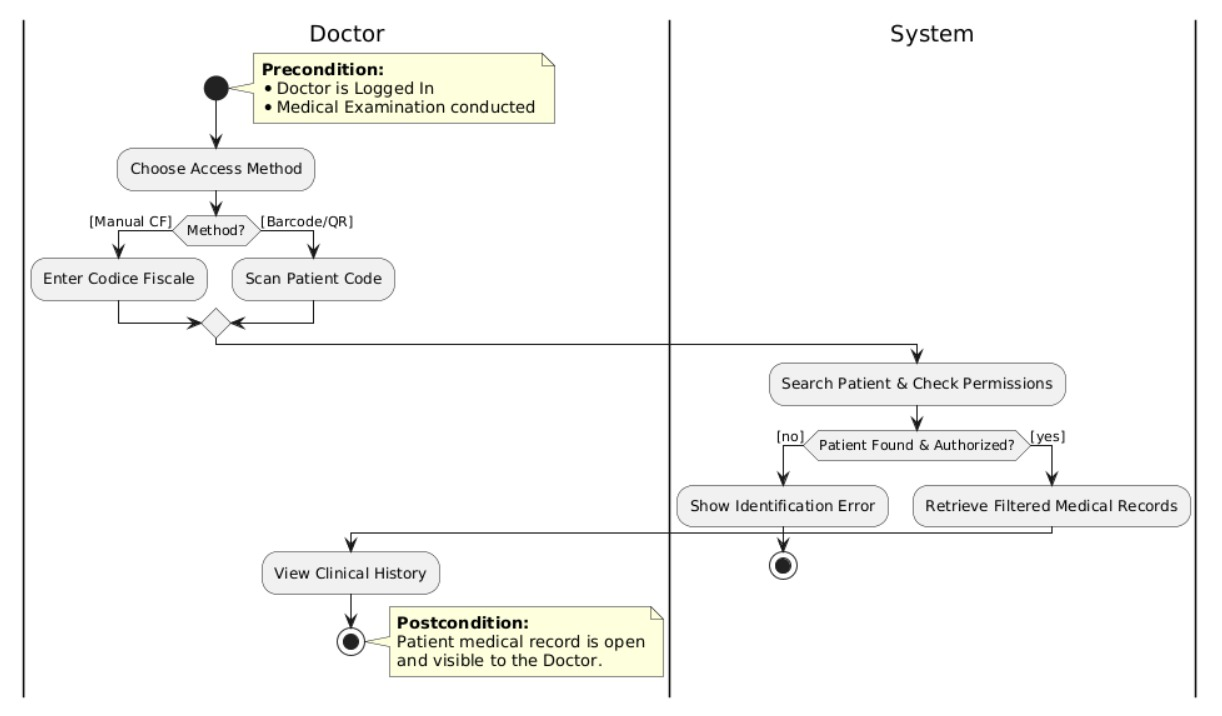
\includegraphics[width=0.8\textwidth]{Activity_Diagram/DoctorMedicalRecord.jpeg}
        \captionof{figure}{Activity Diagram regarding Doctor Accessing Patient's Medical Record}
    \end{center}

    \textbf{Using:} 
    
    \begin{itemize}
        \item \textbf{UC42} Medical record access (Doctor) ,
    \end{itemize}
\end{minipage}
\vspace{3em}

\begin{ucedits}
Following review of D2 the activity diagram number 6 was split to better reflect use cases.
\end{ucedits}



\phantomsection
\begin{minipage}{\textwidth}
    \phantomsection
    \subsection{Activity Diagram 6.2. Doctor uploads Prescription / Exemption / Examination}
    The following activity diagram shows the entire flow of uploading a prescription, exemption, or examination from the doctor's perspective.
    \begin{center}
        
\includegraphics[width=0.8\textwidth]{Activity_Diagram/DoctorUploads.jpeg}
        \captionof{figure}{Activity Diagram regarding Doctor Uploading Prescription / Exemption / Examination}
    \end{center}

    \textbf{Using:} 

    \begin{itemize}
        \item \textbf{UC3} Create Prescription / Exemption,
        \item \textbf{UC4} Upload Examination,    
    \end{itemize}

    
\end{minipage}
\vspace{3em}

\begin{ucedits}
Following review of D2 the activity diagram number 6 was split to better reflect use cases.
\end{ucedits}


\phantomsection
\begin{minipage}{\textwidth}
    \subsection{Activity Diagram 8. Patient Cancel and reschedule appointment}
    The following activity diagram shows the entire flow of cancellation and rescheduling of an appointment from the patient's perspective.
    \begin{center}
        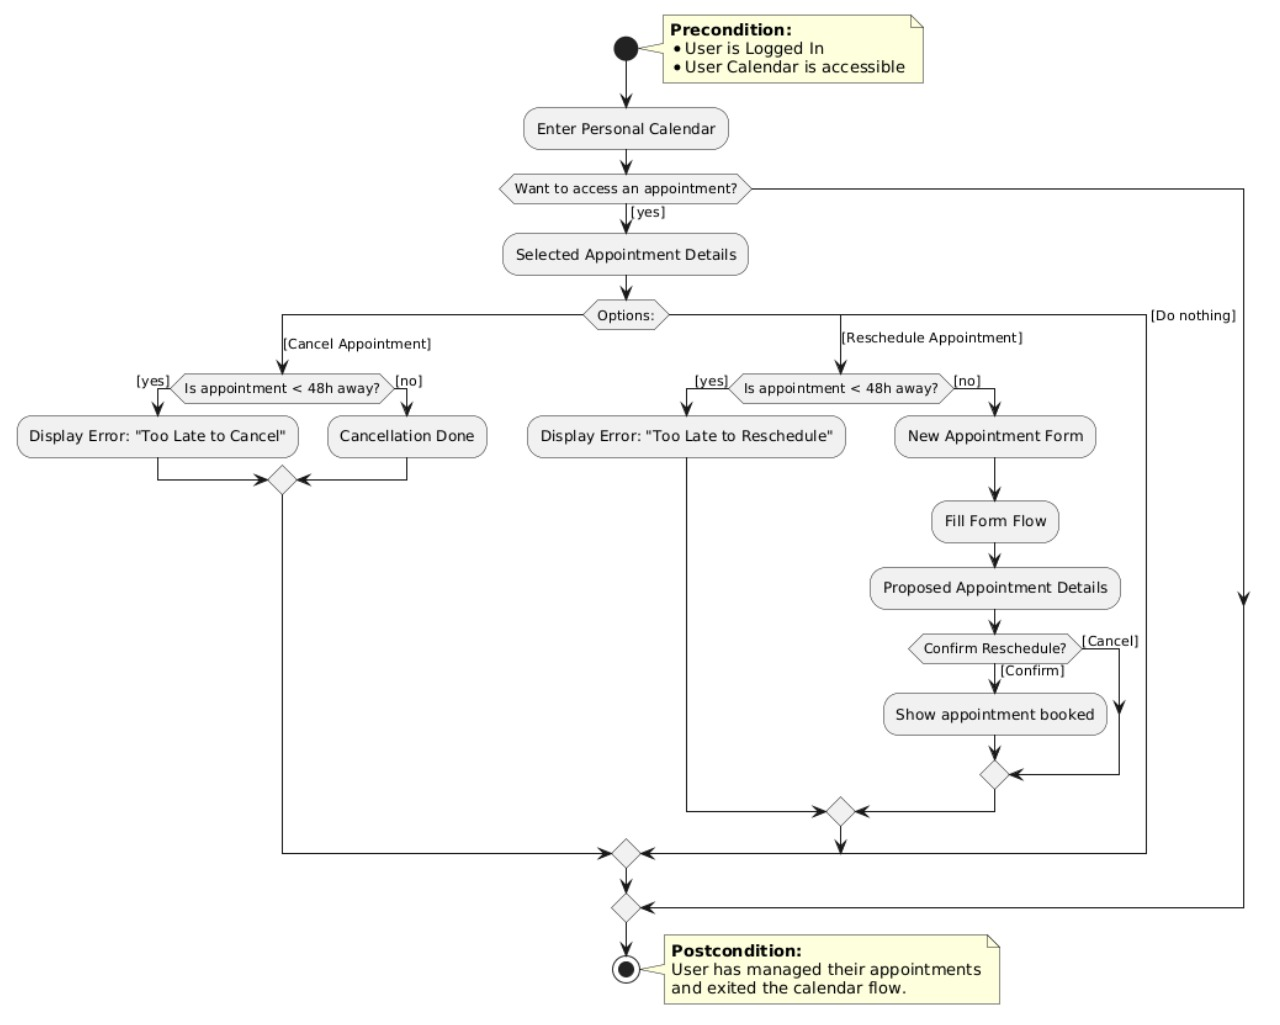
\includegraphics[width=0.8\textwidth]{Activity_Diagram/PatientCancelReschedule.jpeg}
        \captionof{figure}{Activity Diagram regarding Patient Cancel and reschedule appointment}
    \end{center}
    
    \textbf{Using:} 

    \begin{itemize}
        \item \textbf{UC10} Cancel Appointment (Patient),
        \item \textbf{UC29} Appointment rescheduling,
    \end{itemize}
\end{minipage}
\vspace{3em}

\begin{ucedits}
Following review of D2 this activity diagram was added to visualize the steps of the respective use cases.
\end{ucedits}

\phantomsection
\begin{minipage}{\textwidth}
    \subsection{Activity Diagram 9. Patient Medical record and Prescriptions consultation}
    The following activity diagram shows the entire flow of patient medical record access and prescription consultation.
    \begin{center}
        
\includegraphics[width=0.8\textwidth]{Activity_Diagram/PatientMedicalRecordPrescriptions.jpeg}
        \captionof{figure}{Activity Diagram regarding Patient Medical record and Prescriptions consultation}
    \end{center}
    
    \textbf{Using:} 
    
    \begin{itemize}
        \item \textbf{UC38} Prescription Consultation,
        \item \textbf{UC39} Detailed Prescription Access,    
        \item \textbf{UC40} Medical Record Access,    
    \end{itemize}
    
\end{minipage}
\vspace{3em}

\begin{ucedits}
Following review of D2 this activity diagram was added to visualize the steps of the respective use cases.
\end{ucedits}\

\phantomsection
\subsection{Class Diagram}
The following screenshots present the updated class diagram, organized into logical groups 
based on their relevance to the user flows described in the following sections. Each group highlights a meaningful 
subset of the system's classes and their relationships, rather than representing the diagram 
in its entirety. This grouping aims to improve clarity and readability, making it easier to 
trace the connection between each user flow and the classes involved.
\begin{center}
    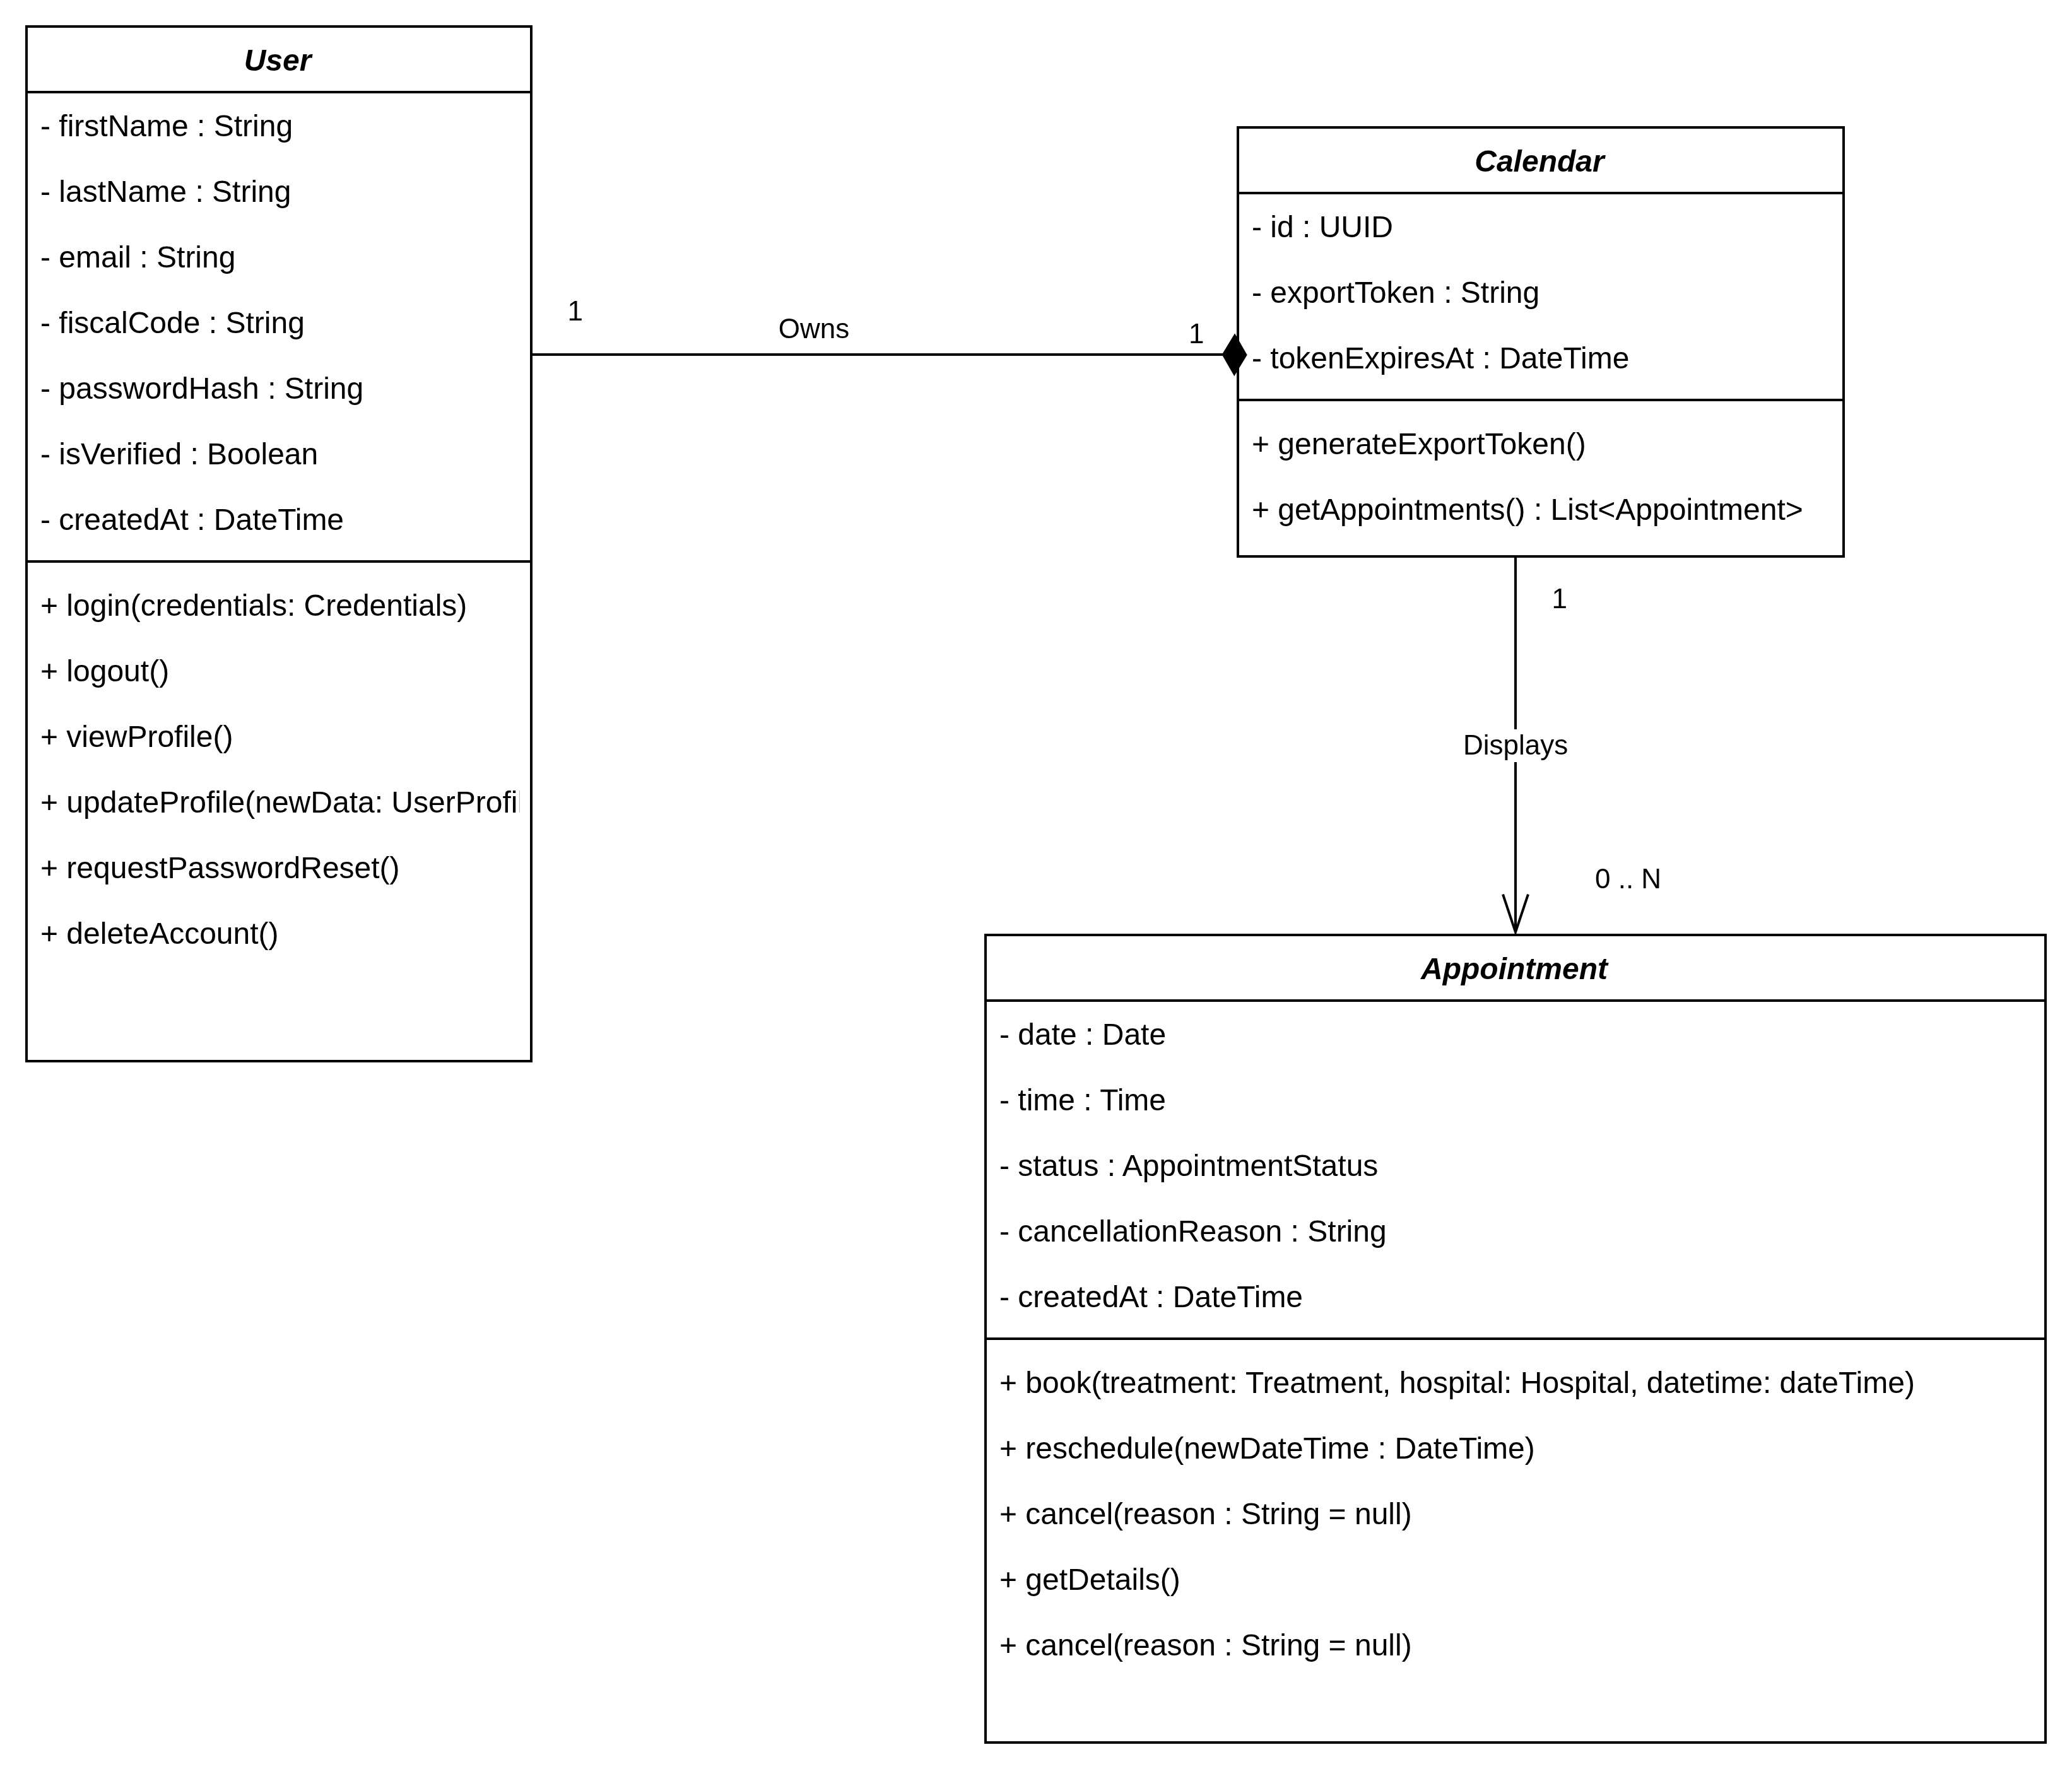
\includegraphics[width=0.9\textwidth, height=0.75\textheight, keepaspectratio]{Class_Diagram/review/genericUser.png}
    \captionof{figure}{Class diagram — Generic User}
\end{center}

\vspace{2em}

\begin{center}
    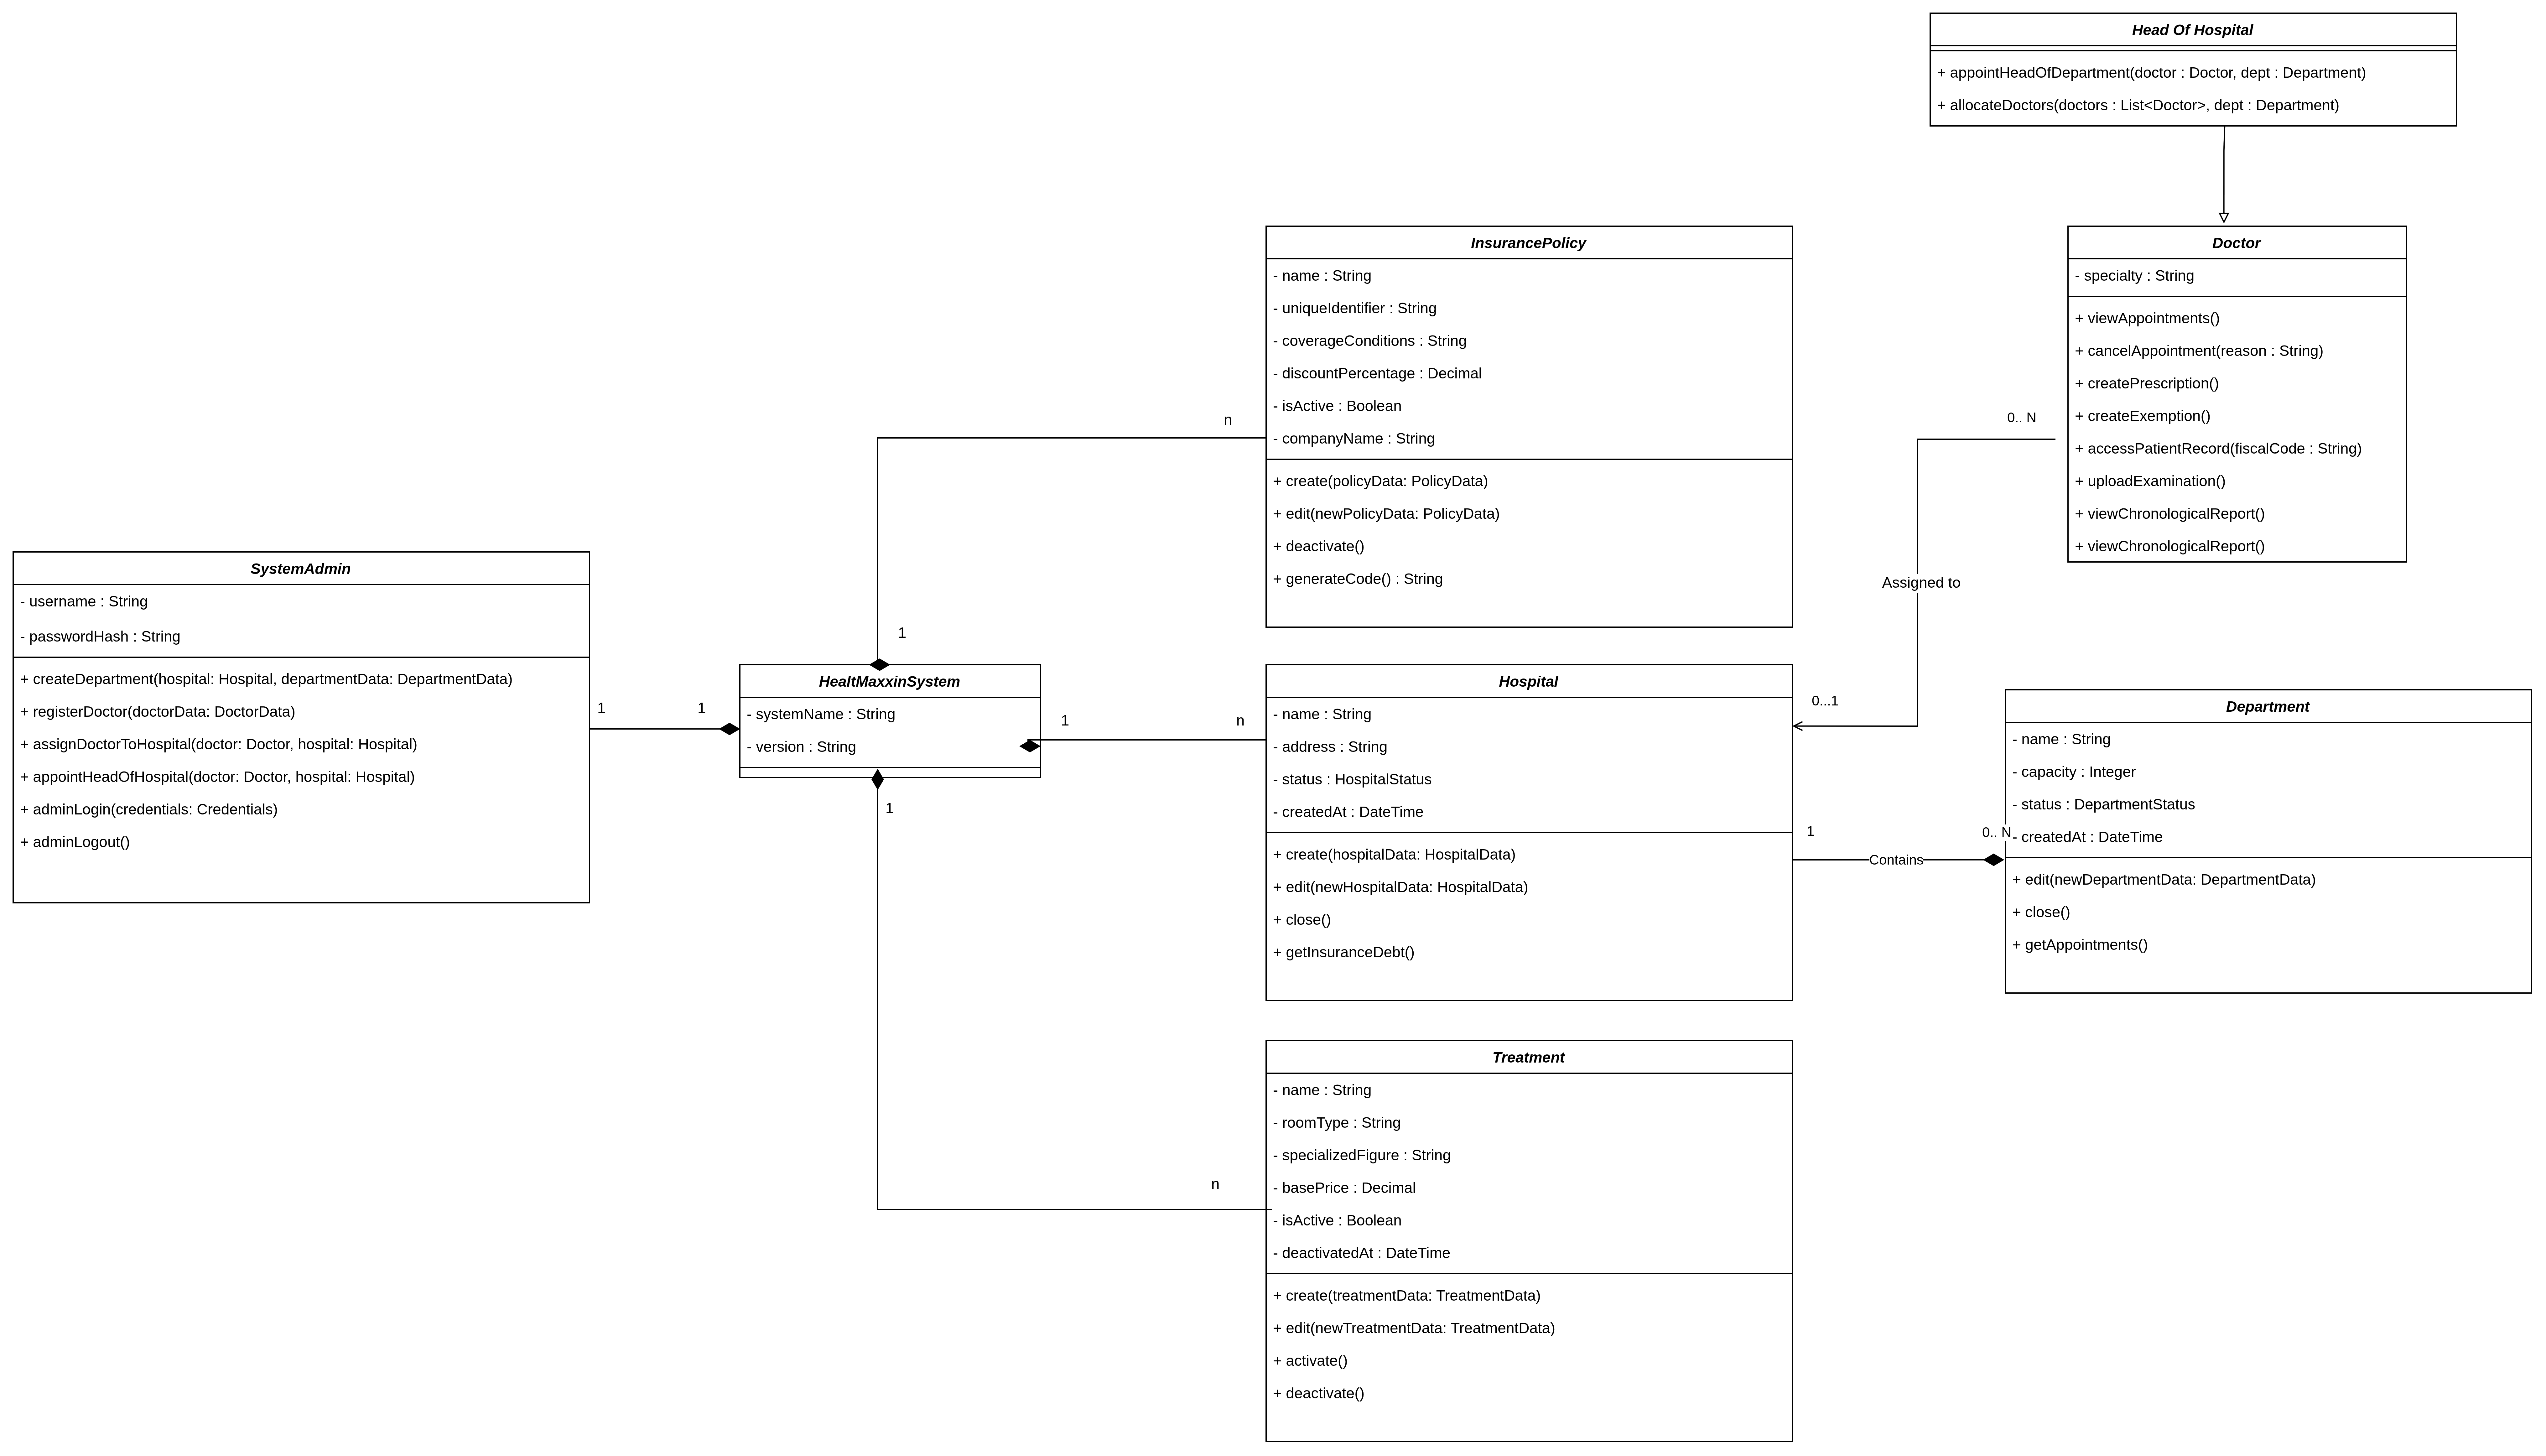
\includegraphics[width=0.9\textwidth, height=0.75\textheight, keepaspectratio]{Class_Diagram/review/admin.png}
    \captionof{figure}{Class diagram — Admin}
\end{center}

\vspace{3em}
\begin{center}
    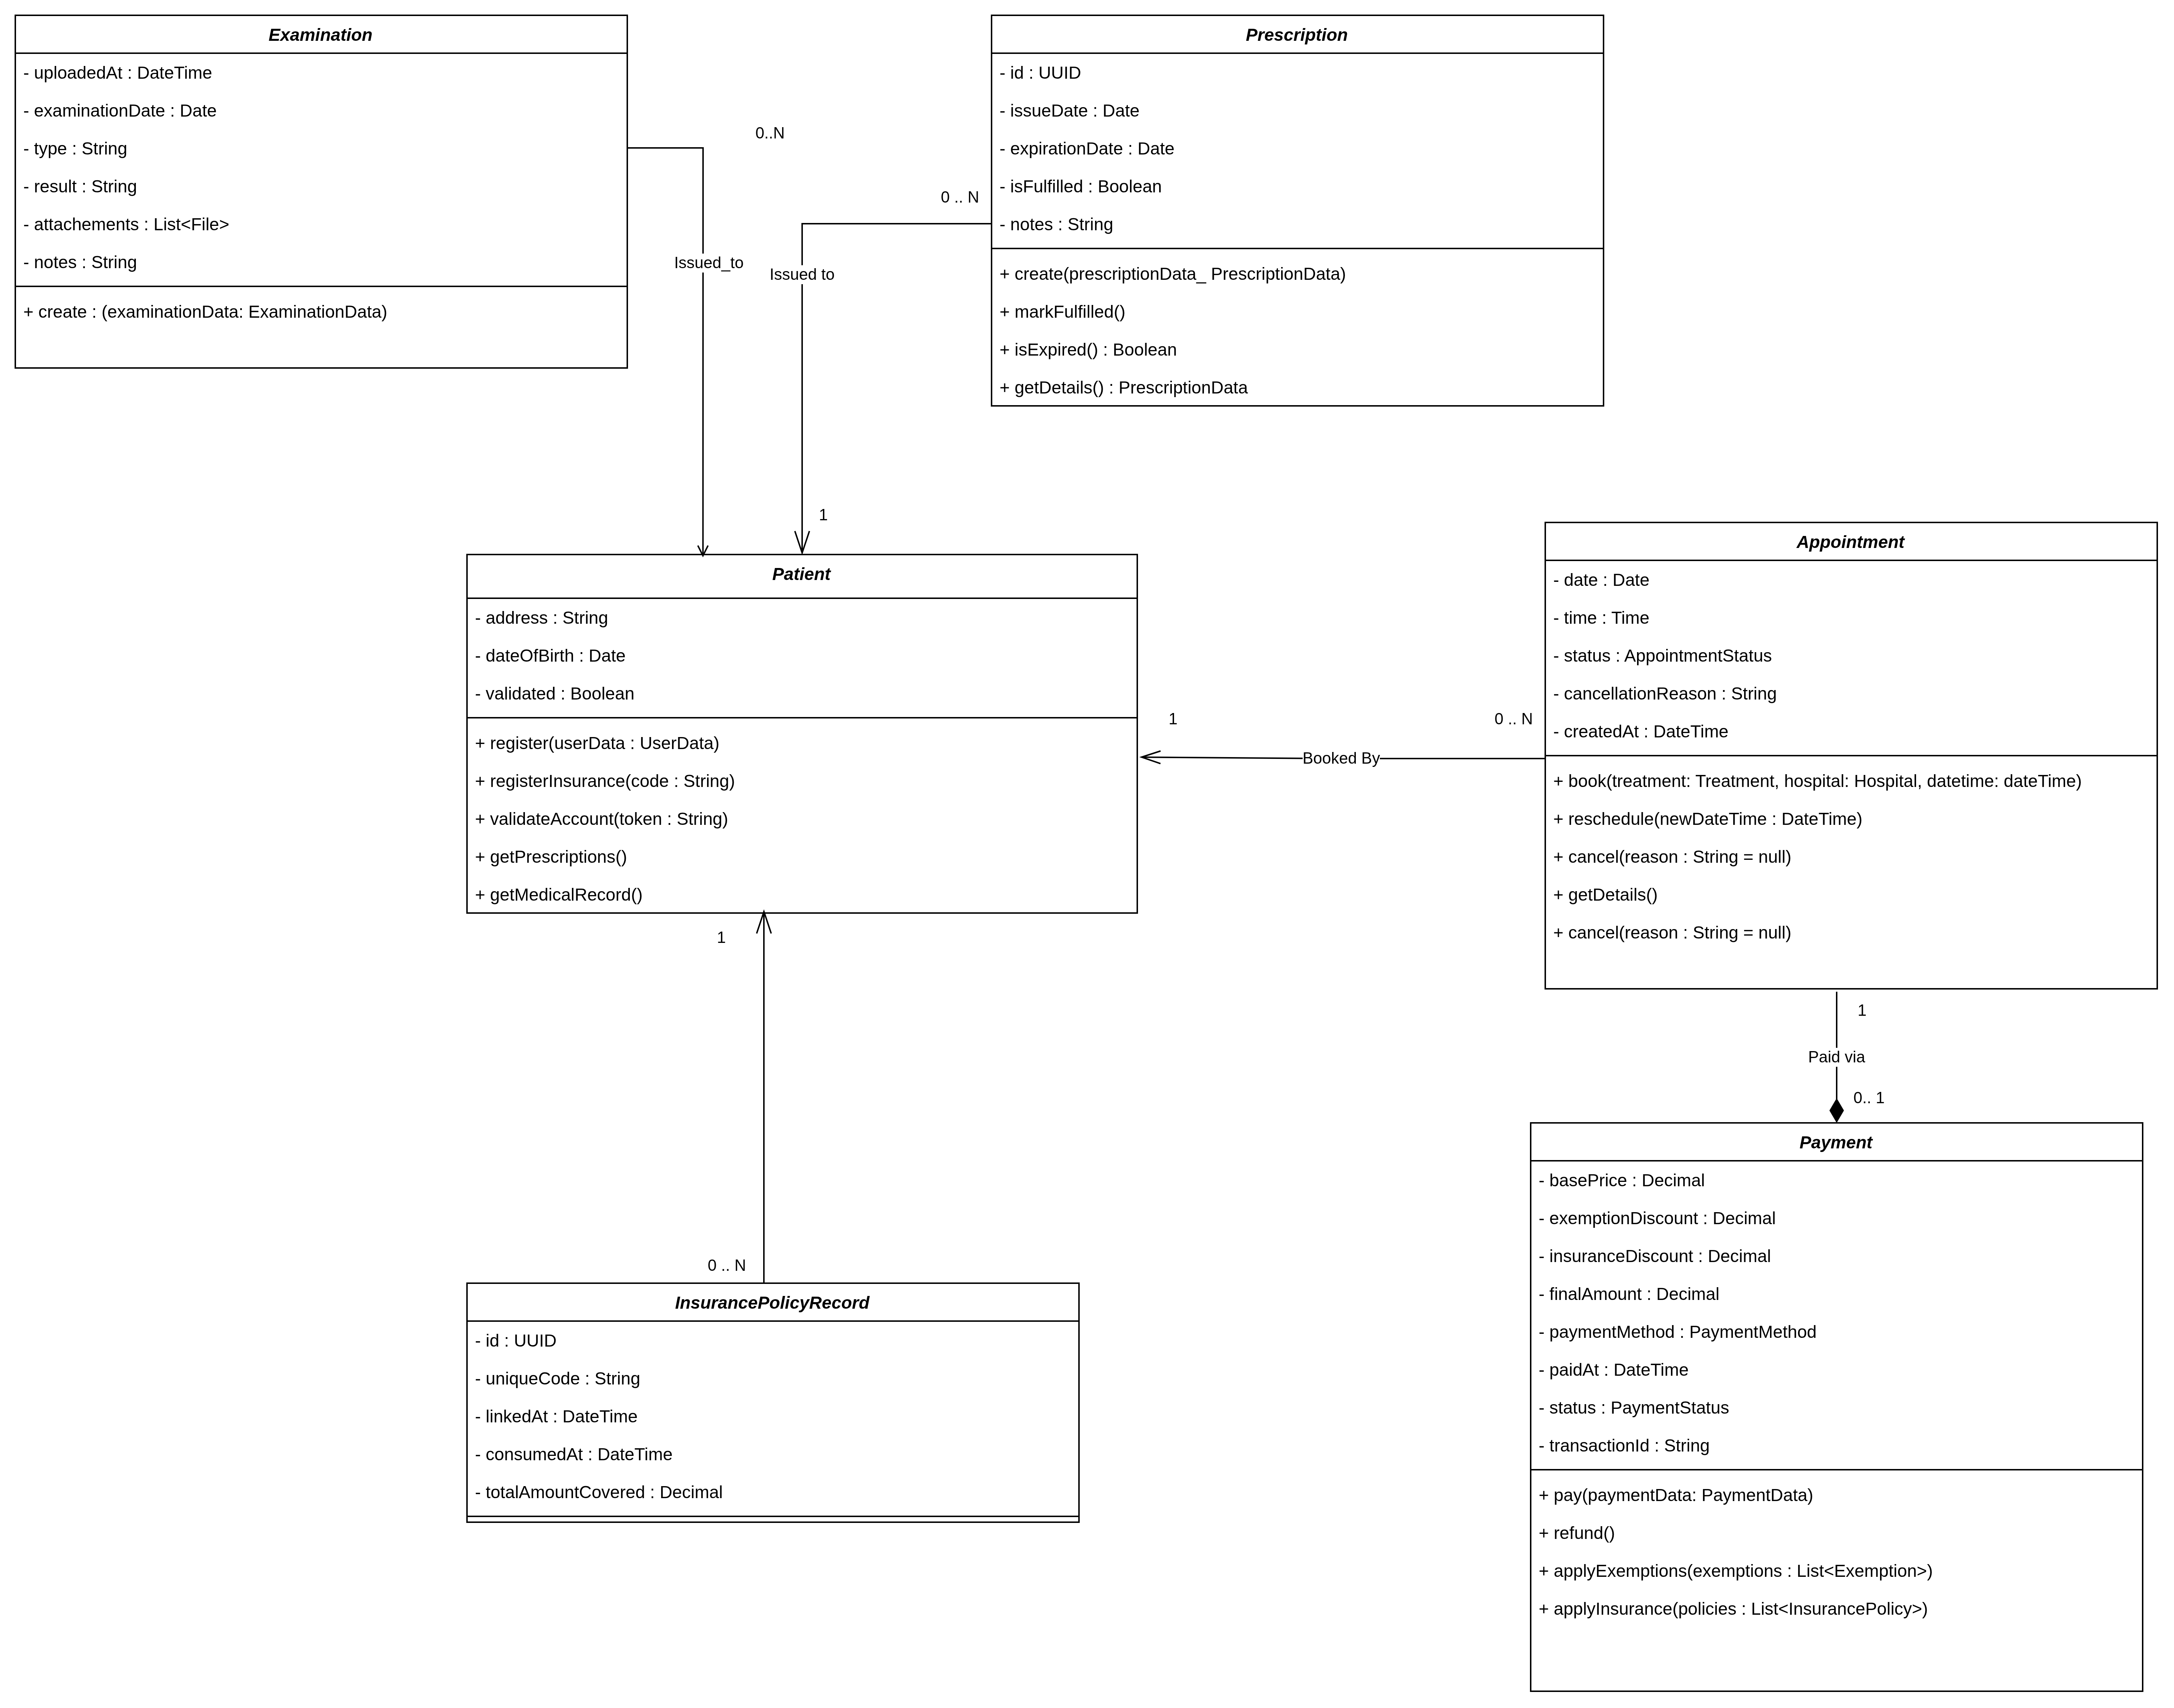
\includegraphics[width=0.9\textwidth, height=0.75\textheight, keepaspectratio]{Class_Diagram/review/patient.png}
    \captionof{figure}{Class diagram — Patient}
\end{center}

\vspace{3em}

\begin{center}
    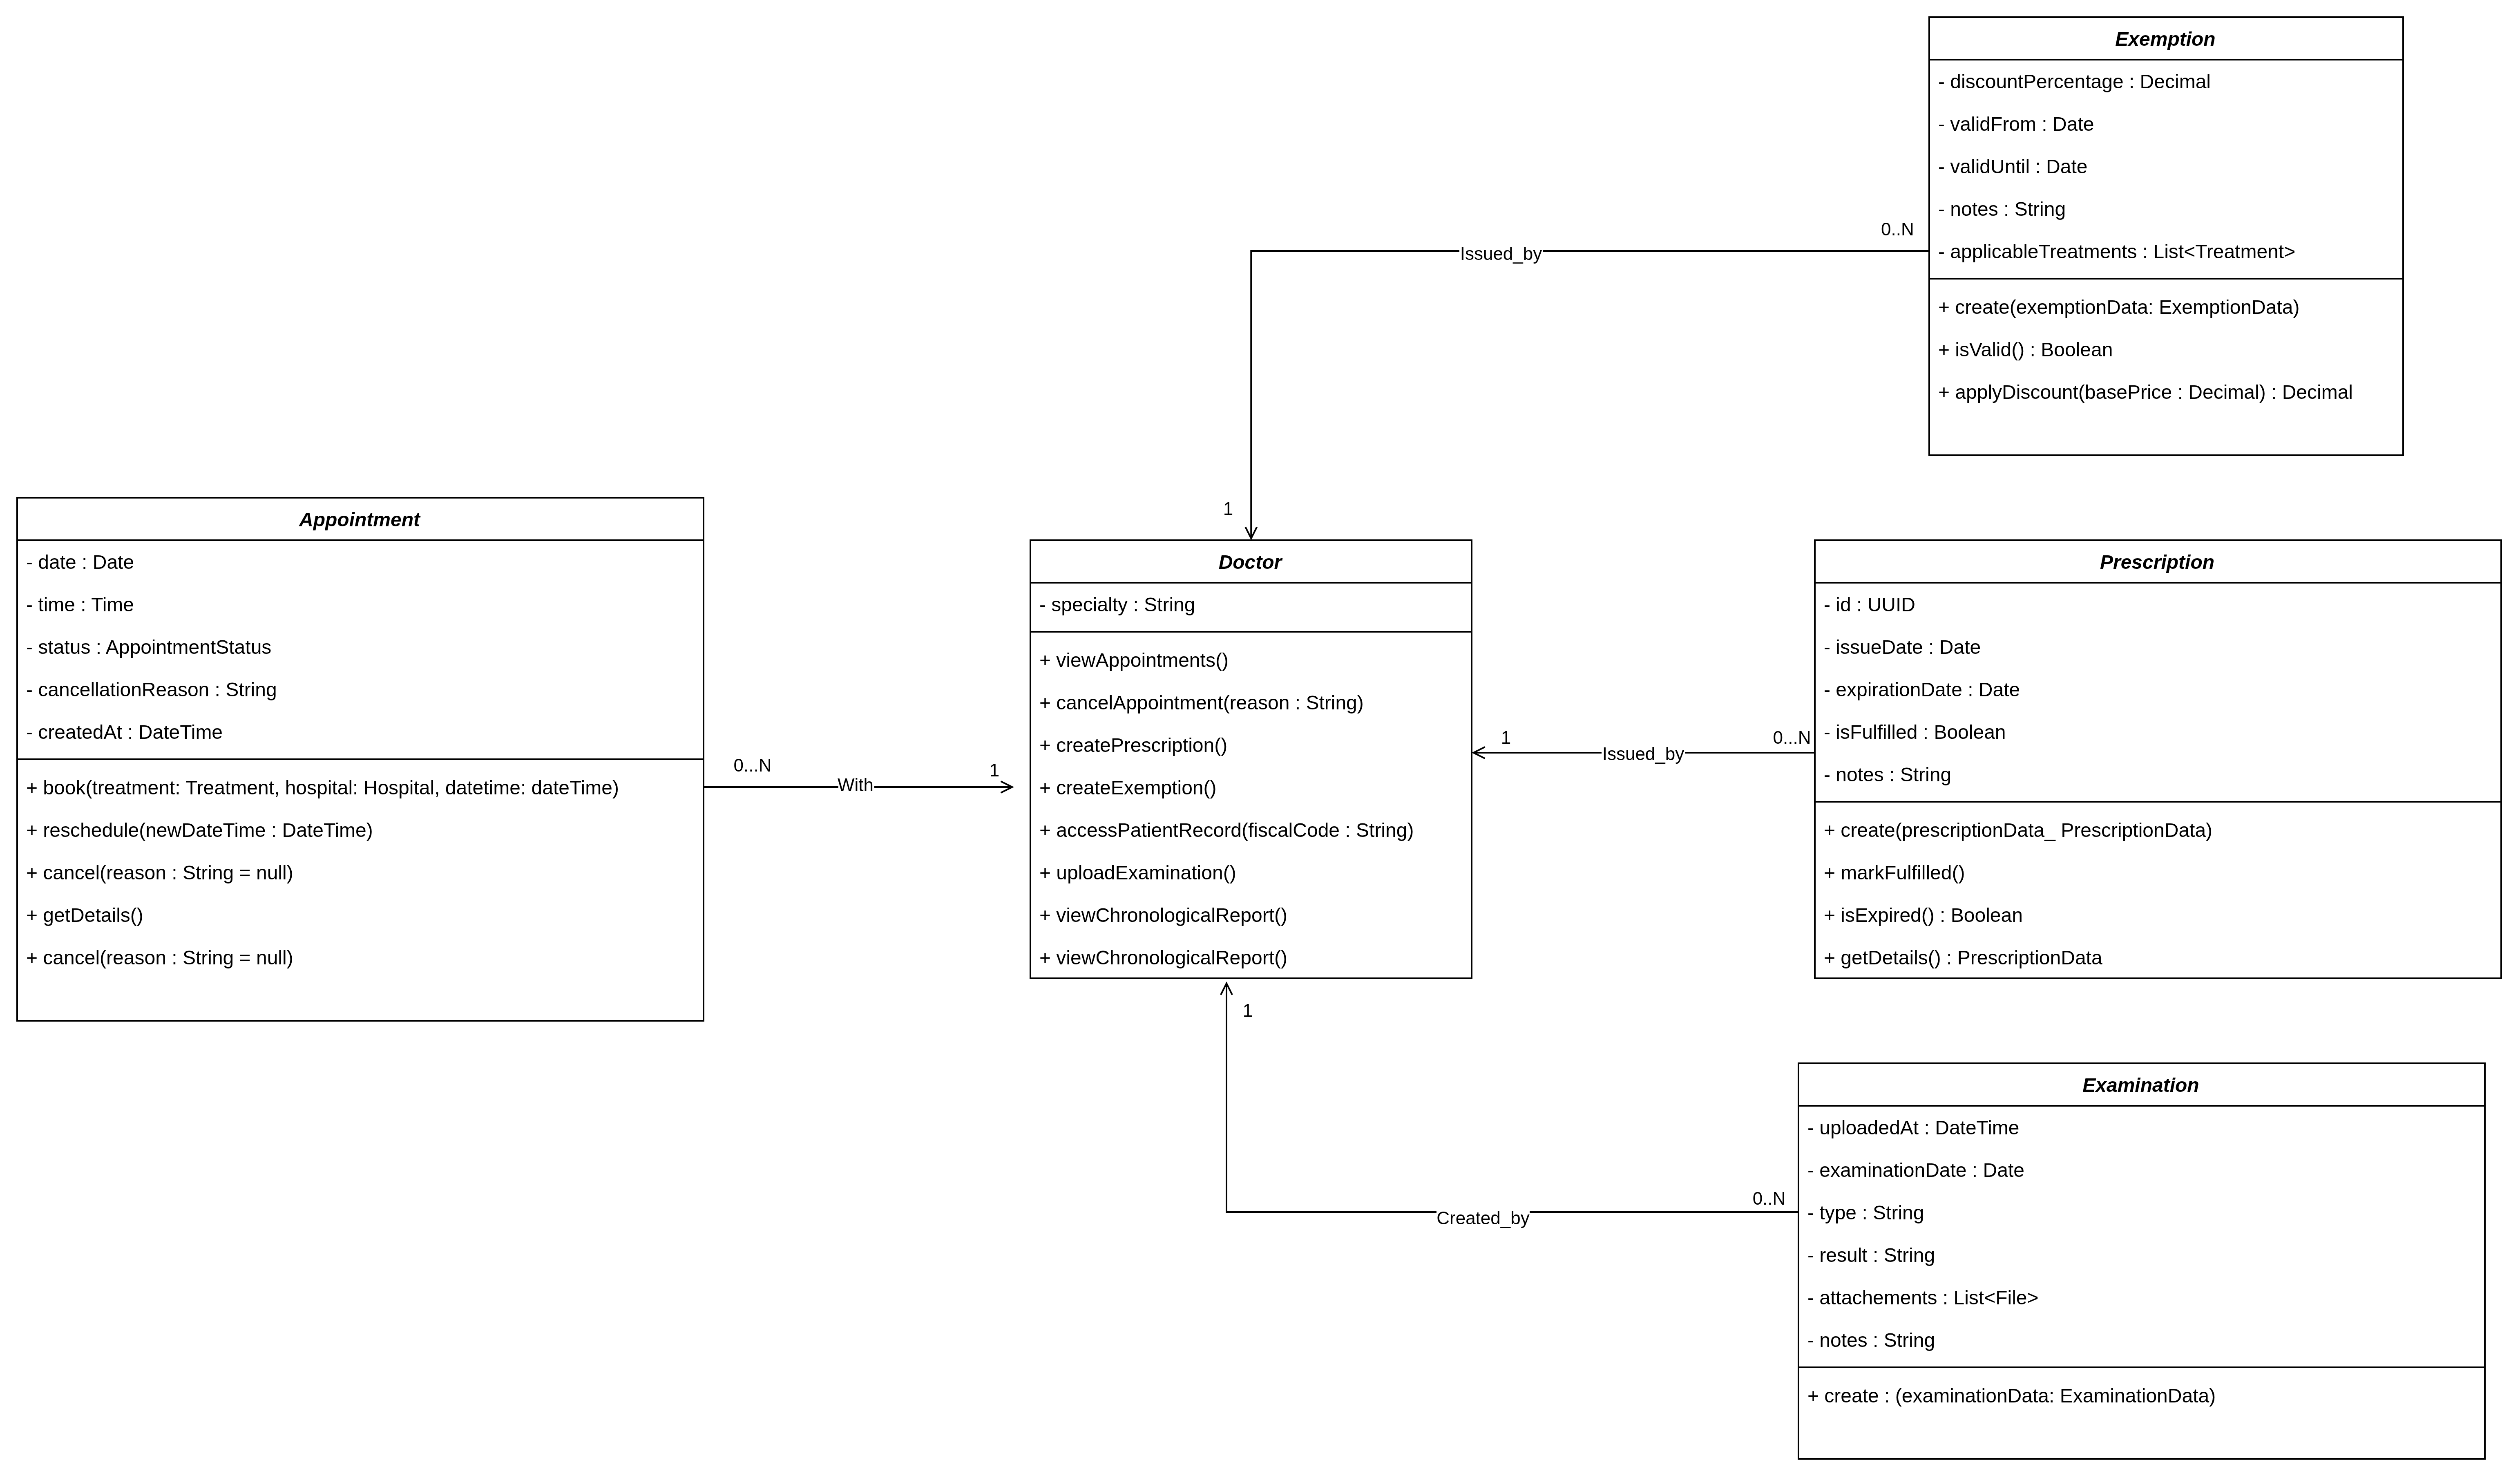
\includegraphics[width=0.9\textwidth, height=0.75\textheight, keepaspectratio]{Class_Diagram/review/doctor.png}
    \captionof{figure}{Class diagram — Doctor}
\end{center}
\begin{center}
    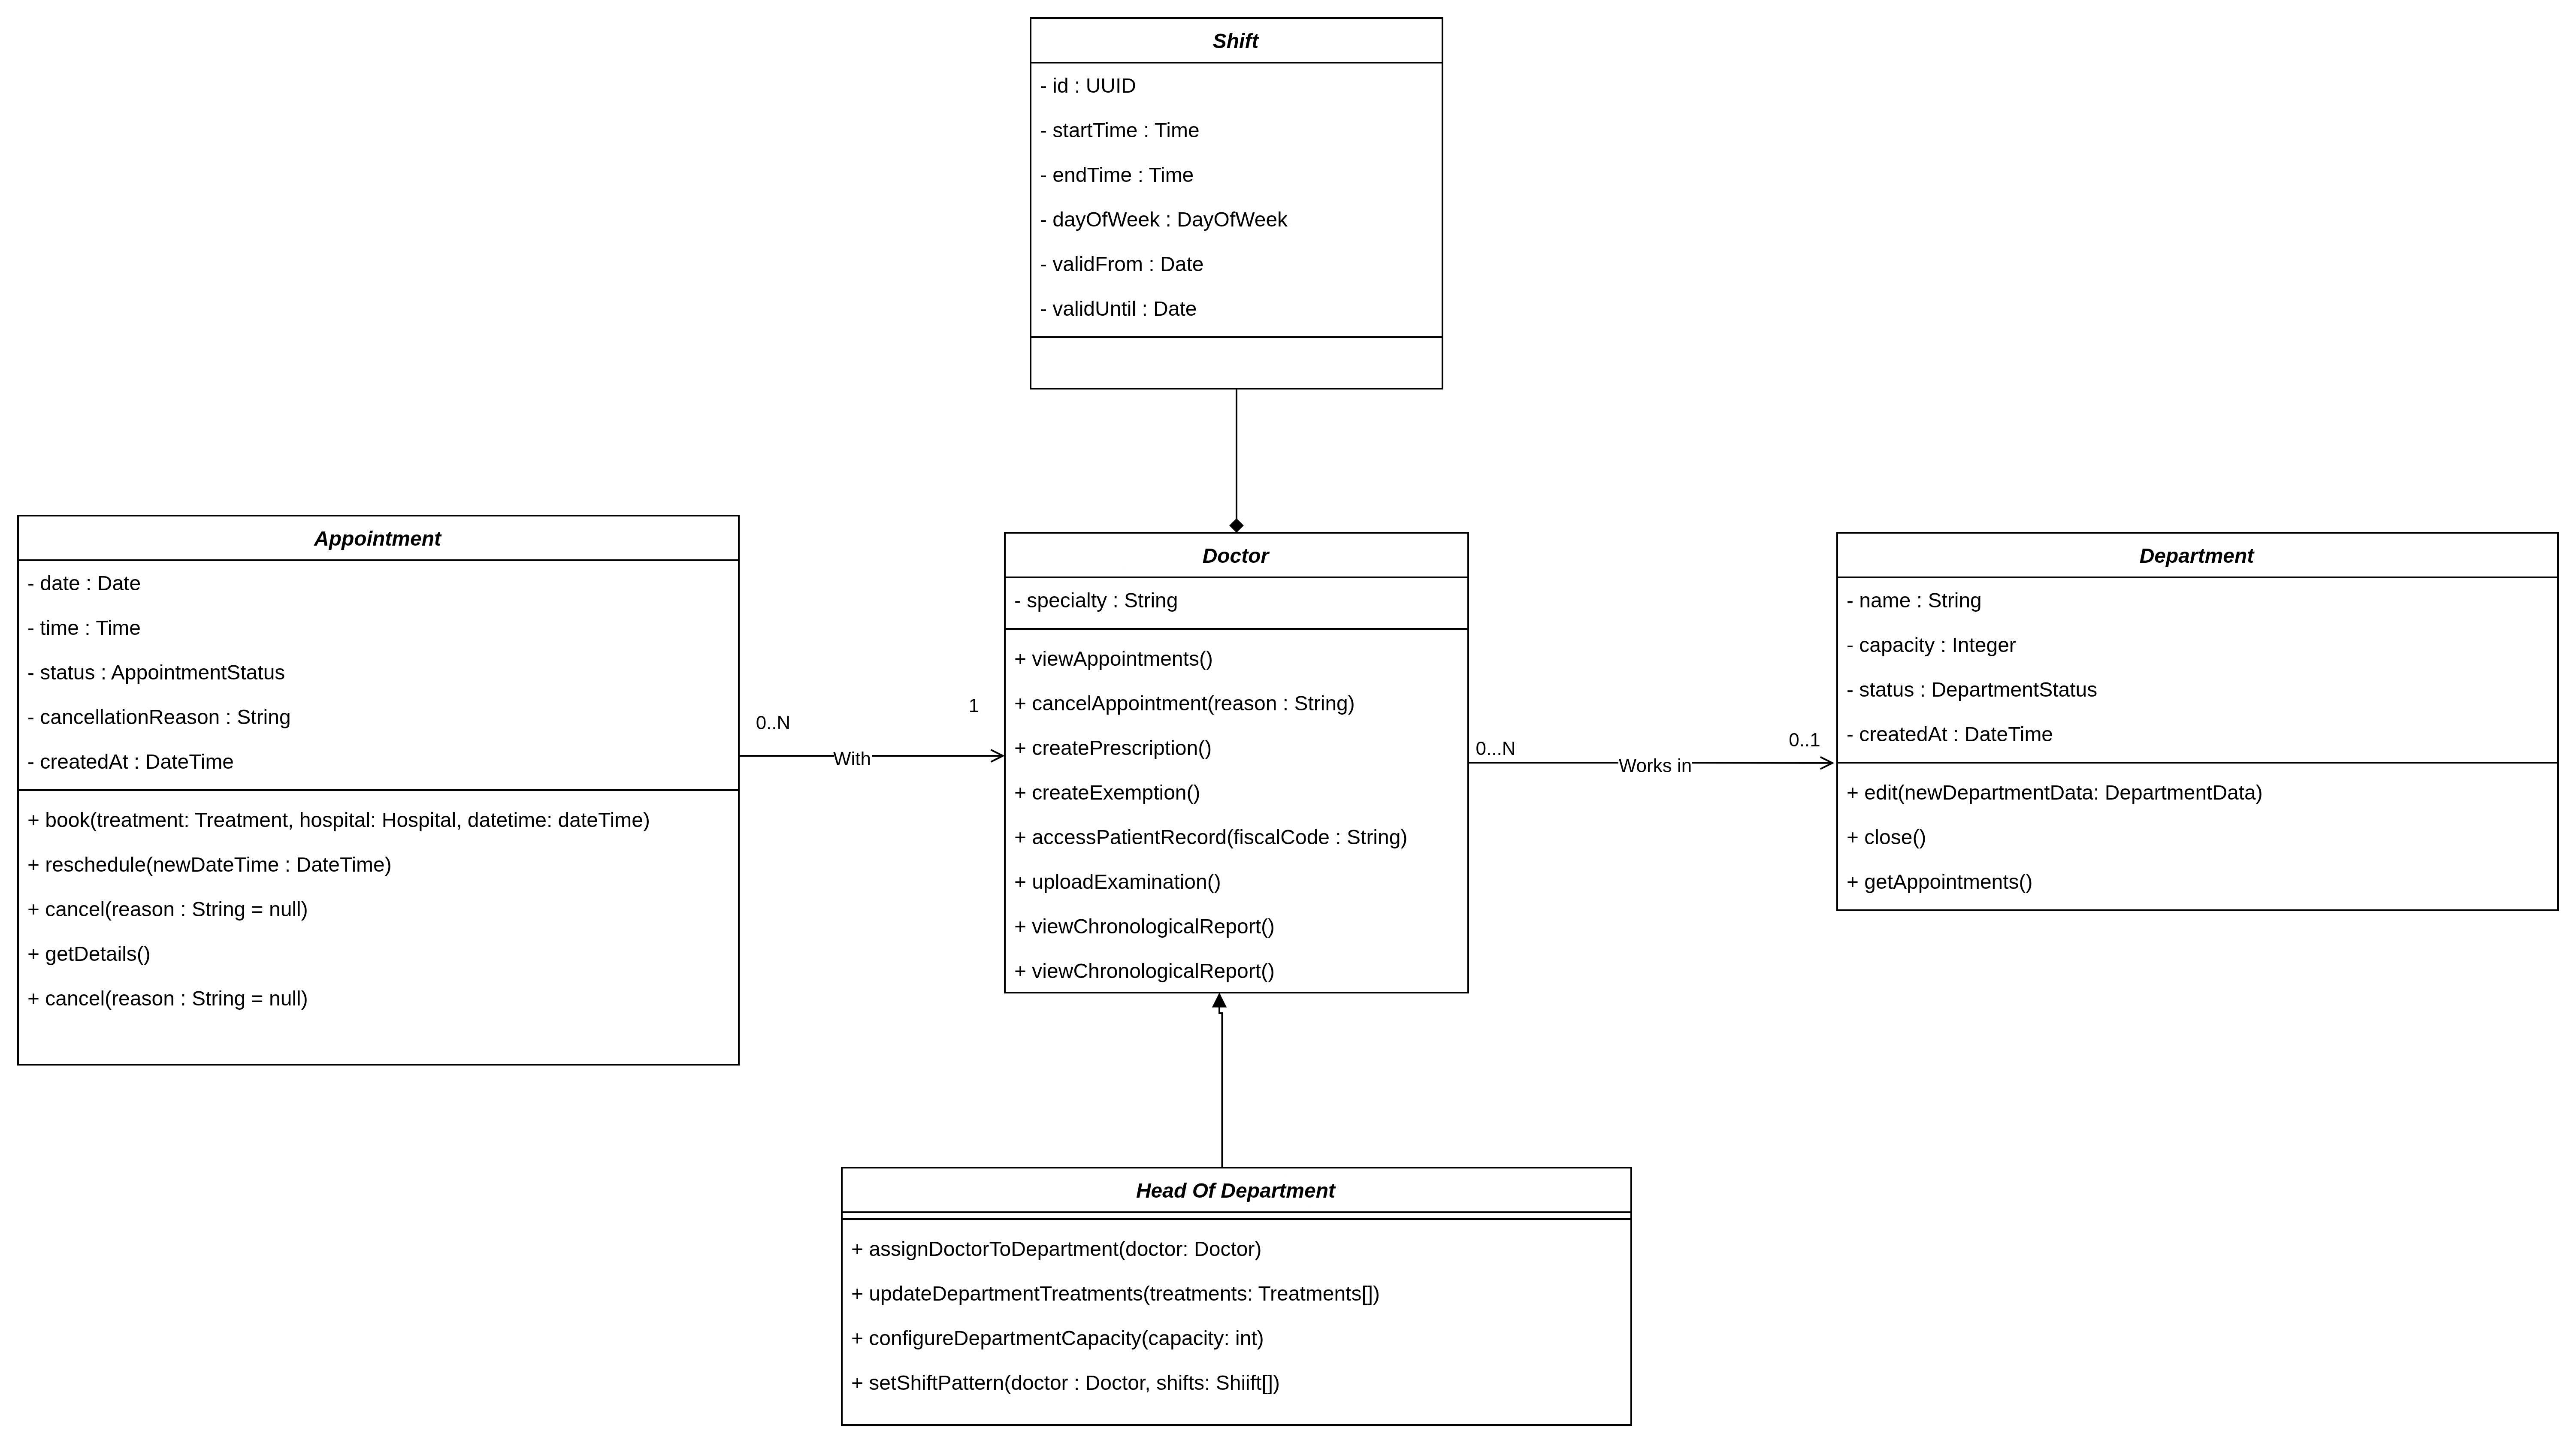
\includegraphics[width=0.9\textwidth, height=0.75\textheight, keepaspectratio]{Class_Diagram/review/headOfDepartment.png}
    \captionof{figure}{Class diagram — Head of Department}
\end{center}
\begin{center}
    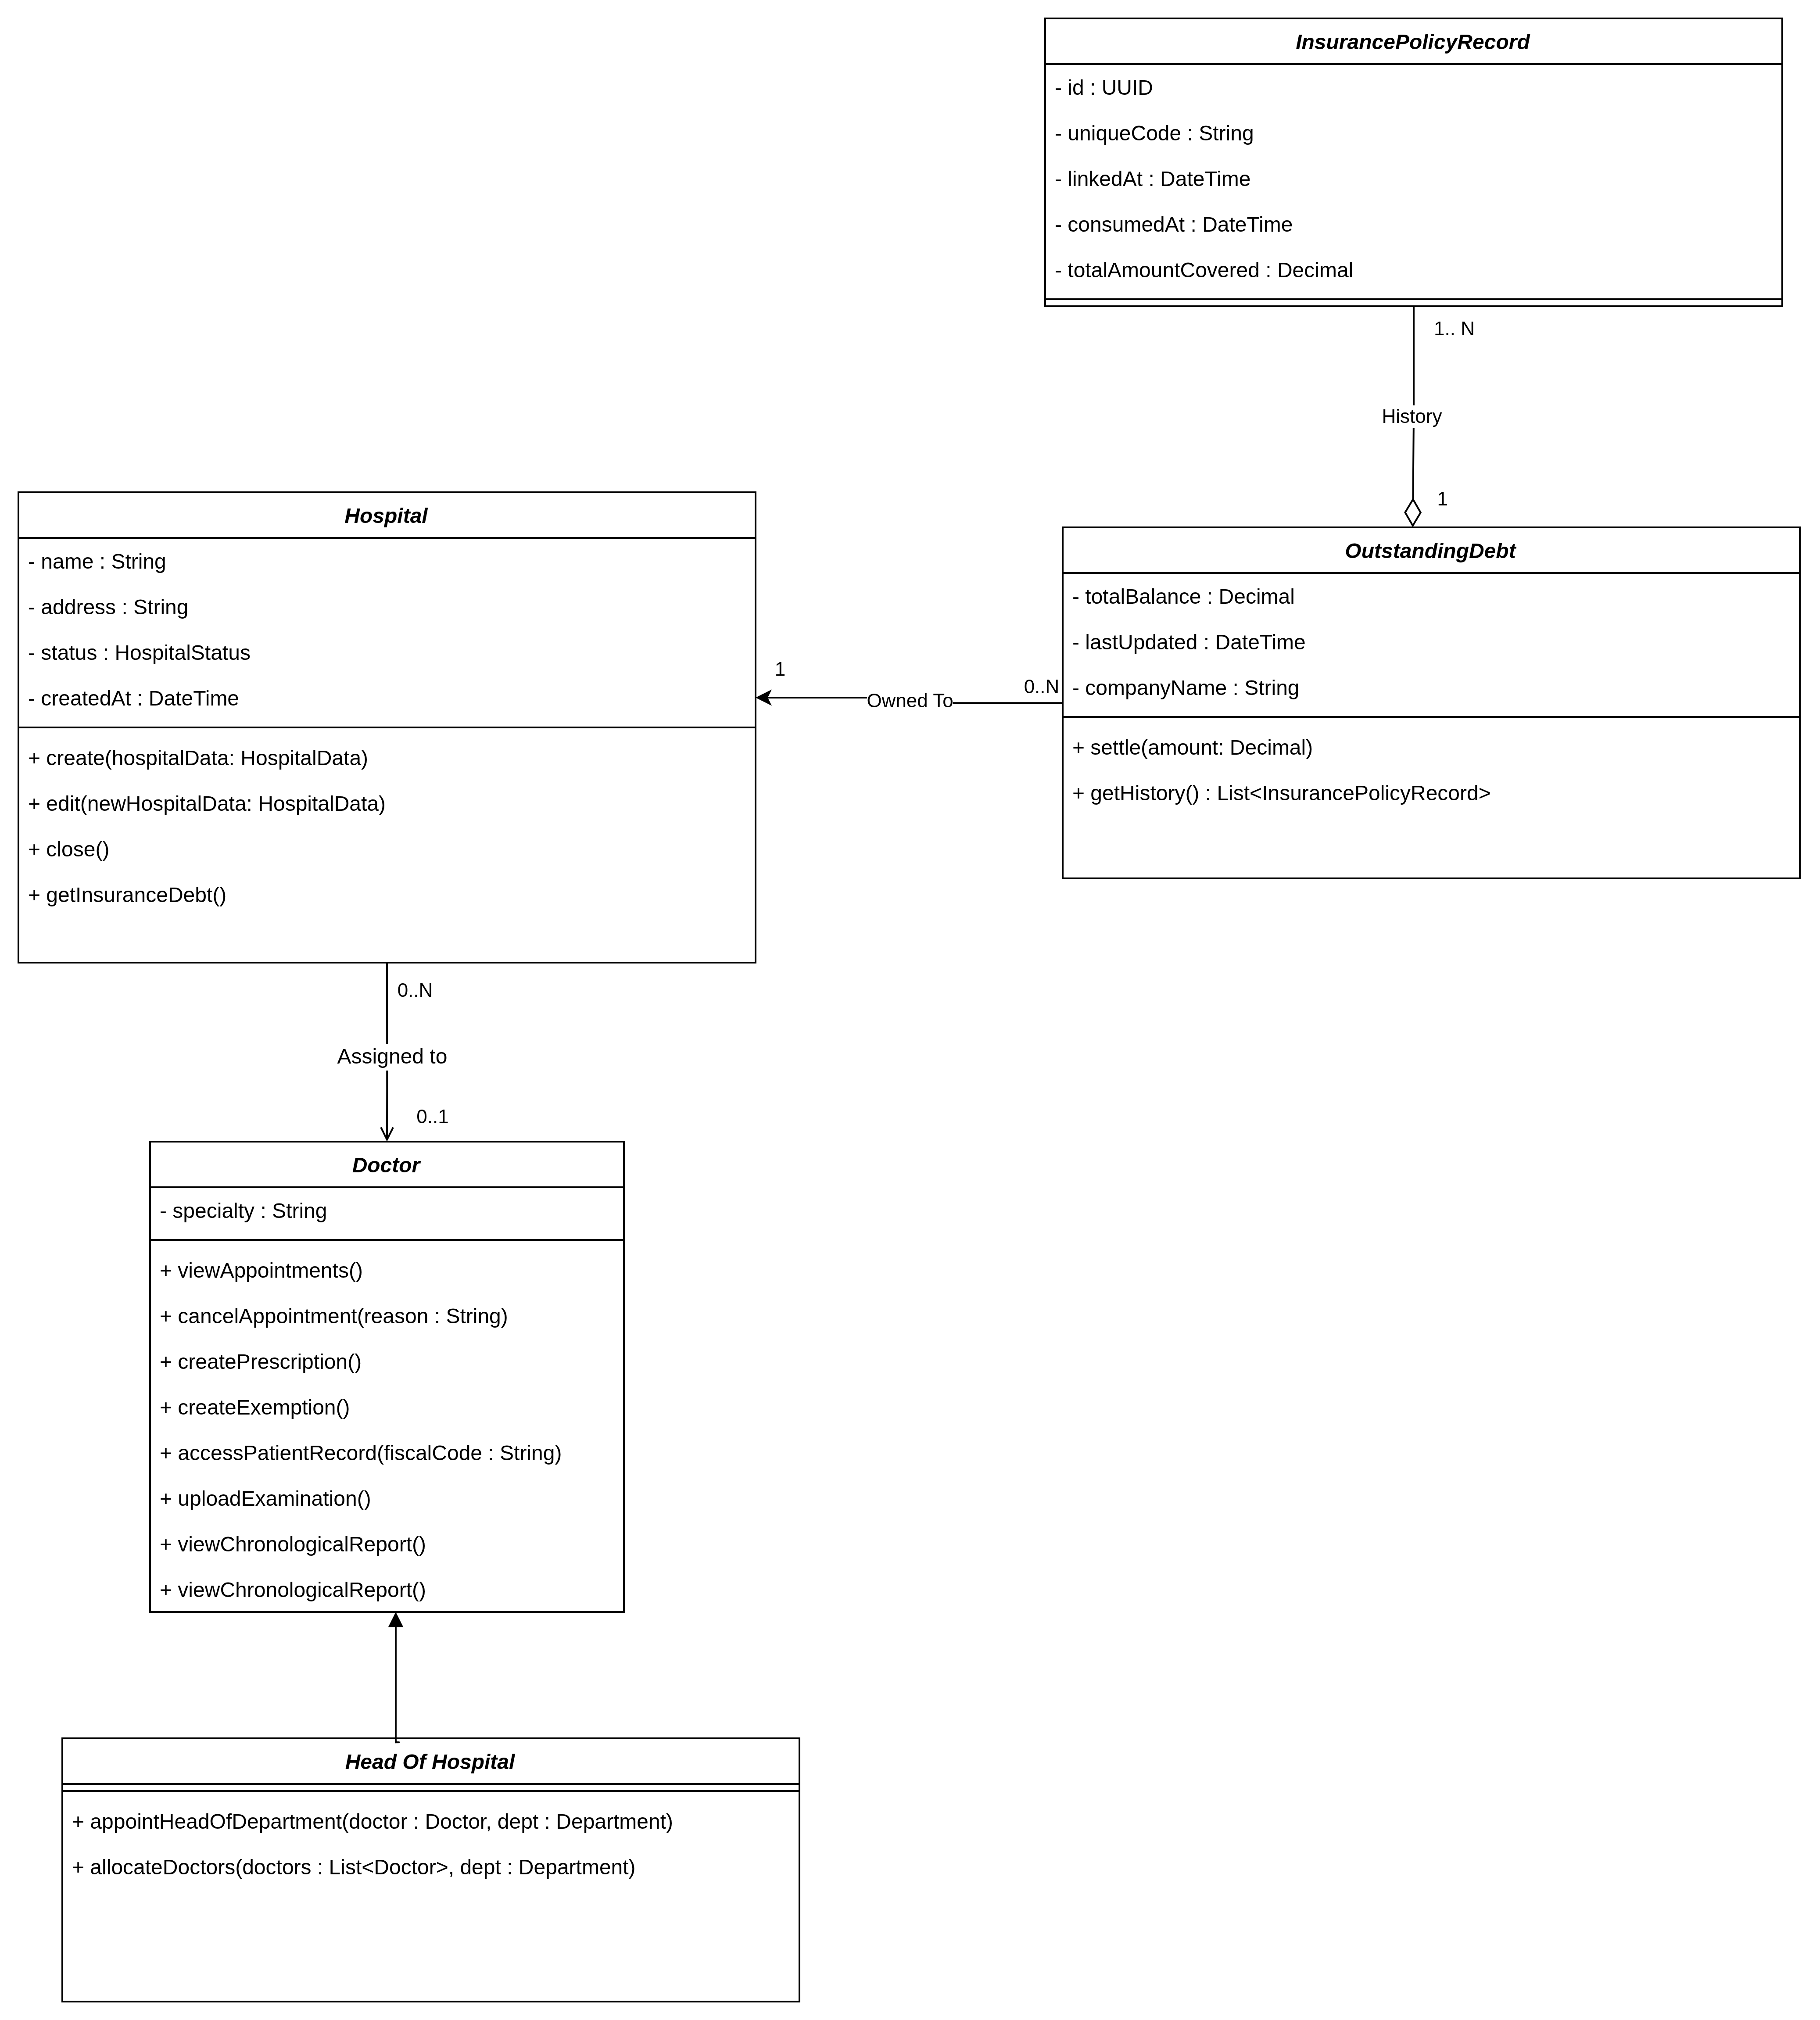
\includegraphics[width=0.9\textwidth, height=0.75\textheight, keepaspectratio]{Class_Diagram/review/headOfHospital.png}
    \captionof{figure}{Class diagram — Head of Hospital}
\end{center}



\vspace{3em}


